\section{Conception : mesurer hors arbre, puis corriger}

\subsection{Mesurer l'\'evaluateur hors arbre}

L'arbre cache la cause : quand la recherche ralentit, on ne sait pas si c'est
la collecte, la forme du lot, le buffer ou le GPU. Le premier livrable du
chantier est donc un banc qui appelle \code{evaluate\_batch} directement, sur
des tenseurs al\'eatoires, sans arbre.

\begin{mesure}[Protocole du banc \'evaluateur]
\begin{itemize}[leftmargin=1.2em,itemsep=2pt]
  \item lots fixes balay\'es de 1 \`a 256, avec \'echauffement, 30
  r\'epetitions et 20 appels par mesure ; les lots 3, 5, 6, 7, 12, 24, 48 et
  96 sont mesur\'es dans une seconde campagne ;
  \item un mode \code{--variable} qui alterne les lots 1 \`a 8 \`a chaque
  appel, comme le fait la recherche, et accumule par taille ;
  \item un mode \code{--fake} qui valide le harnais avec
  \code{ControlledEvaluator}, sans mod\`ele ;
  \item deux chronom\`etres internes optionnels, d\'esactiv\'es par d\'efaut en
  production, qui s\'eparent \code{session->Run} du softmax C++.
\end{itemize}
\end{mesure}

Le banc sort un JSON par mesure, agr\'eg\'e ensuite en m\'edianes. Le mod\`ele
et le GPU sont ceux de production, et le provider CUDA est le m\^eme.

\subsection{La d\'ecouverte : la forme du lot}

La figure~\ref{fig:courbe-evaluateur} et le tableau~\ref{tab:evaluateur}
montrent le r\'esultat. En lots fixes, le co\^ut par position d\'ecro\^it de
9,75\,ms (lot 1) \`a 0,10\,ms (lot 128). En lots altern\'es 1 \`a 8, chaque
appel co\^ute 13,5\,ms, dont 13,4\,ms de \code{session->Run}, \emph{quel que
soit le lot}. Le contraste est brutal : la recherche ne payait pas le r\'eseau,
elle payait le changement de forme.

\begin{figure}[h]
\centering
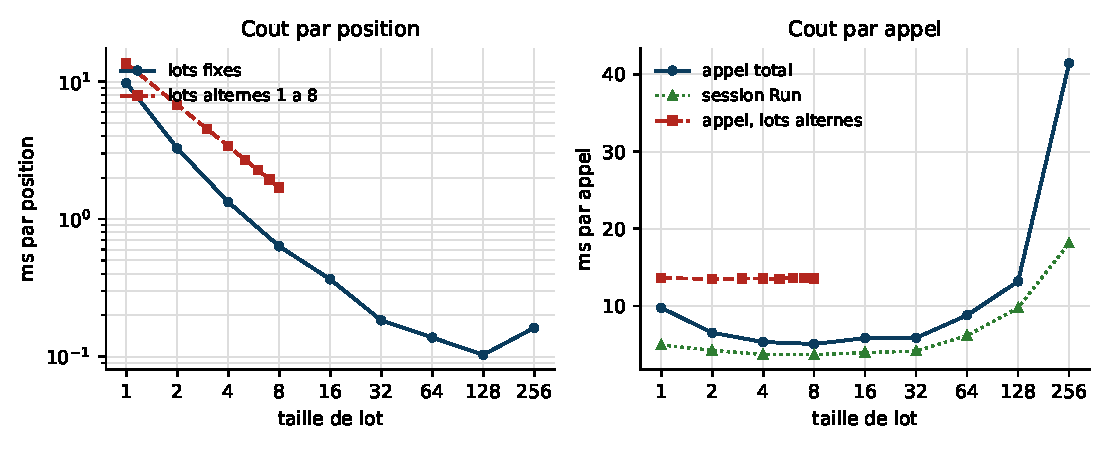
\includegraphics[width=\textwidth]{figures/fig_evaluateur_courbe.pdf}
\caption{Co\^ut de l'\'evaluateur hors arbre, GPU. \`A gauche, le co\^ut par
position en lots fixes (bleu) et en lots altern\'es (rouge). \`A droite, le
co\^ut par appel, avec la part \code{session->Run} en pointill\'es verts.}
\label{fig:courbe-evaluateur}
\end{figure}

\begin{table}[h]
\centering
\small
\caption{Courbe du lot, GPU, lots fixes (m\'edianes).}
\label{tab:evaluateur}
\begin{tabular}{rrrr}
\toprule
Lot & ms par appel & ms par position & run ONNX (ms) \\
\midrule
1 & 9,75 & 9,75 & 4,95 \\
2 & 6,53 & 3,26 & 4,23 \\
4 & 5,32 & 1,33 & 3,71 \\
8 & 5,07 & 0,63 & 3,67 \\
16 & 5,83 & 0,36 & 3,95 \\
32 & 5,86 & 0,18 & 4,15 \\
64 & 8,79 & 0,14 & 6,16 \\
128 & 13,18 & 0,10 & 9,77 \\
256 & 41,43 & 0,16 & 18,12 \\
\bottomrule
\end{tabular}
\end{table}

Les lots partiels mesur\'es isol\'ement (3, 5, 6, 7) co\^utent tous environ
3,4\,ms, \emph{moins} que le lot 8 de la premi\`ere campagne. Autrement dit,
aucune forme prise seule n'est ch\`ere ; c'est leur alternance qui l'est. Un
A/B interleaved serr\'e confirme : 13,03 et 13,04\,ms en alternance contre 2,87
et 3,65\,ms \`a forme fixe 8, soit un facteur quatre.

\begin{piege}[Le pi\`ege : accuser le r\'eseau ou les allocations]
Les allocations par vague et le softmax C++ \'etaient les coupables
d\'esign\'es. Les mesures les innocentent : le softmax vaut 0,02 \`a 0,10\,ms
par appel, soit 0,2 \`a 2\,\%, et retirer les allocations par appel ne
changerait pas l'ordre de grandeur. La cause \'etait le contrat implicite
d'ONNX Runtime : une forme de tenseur stable est un pattern m\'emoire
r\'eutilisable, une forme qui change est un graphe \`a re-planifier.
\end{piege}

\subsection{La correction : lot de forme fixe}

La correction consiste \`a ne plus jamais changer la forme du lot en cours de
recherche. Chaque vague collecte un nombre variable de feuilles
r\'eseau ; le coordinateur duplique le dernier tenseur jusqu'\`a
\code{batch\_size}, appelle l'\'evaluateur avec la forme fixe, puis n'utilise
que les sorties des positions r\'eelles.

\begin{lstlisting}[caption={Padding d'une vague (extrait de \code{mcts\_wave.cpp}).}]
const int eval_batch = m_fixed_batch ? batch_size
                                    : static_cast<int>(network_count);
if (m_fixed_batch && network_count > 0) {
    eval_batch = batch_size;
    const std::size_t target = batch_size * TENSOR_SIZE;
    if (batch_input.size() < target) {
        batch_input.reserve(target);
        const std::vector<float> dernier(
            batch_input.end() - TENSOR_SIZE, batch_input.end());
        while (batch_input.size() < target) {
            batch_input.insert(batch_input.end(),
                               dernier.begin(), dernier.end());
        }
    }
}
\end{lstlisting}

Trois choix de conception m\'eritent d'\^etre explicit\'es.

\textbf{Pourquoi dupliquer le dernier tenseur plut\^ot que des z\'eros.} Une
rang\'ee dupliqu\'ee co\^ute le m\^eme temps GPU qu'une rang\'ee r\'eelle, mais
elle ne demande aucun remplissage suppl\'ementaire et le tenseur est d\'ej\`a
contigu dans le buffer. Le contenu n'a aucune importance puisque la sortie est
ignor\'ee.

\textbf{Pourquoi laisser la racine au lot 1.} L'expansion de racine est un
appel unique par coup, avec un seul tenseur. La padder \`a 8 gaspillerait sept
\'evaluations par coup pour rien. Il reste donc deux formes dans une recherche,
1 puis 8 : la premi\`ere vague apr\`es la racine paie une re-planification,
n\'egligeable sur un coup entier.

\textbf{Pourquoi la recherche est s\'emantiquement inchang\'ee.} Les positions
r\'eelles occupent les indices 0 \`a \code{network\_count-1} du lot, avant et
apr\`es le padding ; la sortie d'une rang\'ee ne d\'epend pas des autres
rang\'ees, le softmax \'etant calcul\'e par position. Chaque feuille r\'eelle
re\c coit donc exactement la policy et la value qu'elle aurait eues sans
padding. Seules changent la taille du tenseur d'entr\'ee et les rang\'ees
suppl\'ementaires, dont les sorties sont jet\'ees.

\subsection{Les alternatives \'ecart\'ees}

\begin{table}[h]
\centering
\small
\caption{Pistes examin\'ees et verdict.}
\label{tab:alternatives}
\begin{tabularx}{\textwidth}{lXl}
\toprule
Piste & Raison & Verdict \\
\midrule
Buffers persistants & Le facteur dominant est la forme, pas l'allocation ;
les vagues allouent environ 200 kio par appel, soit moins de 1\,\% & non retenue \\
IO binding, CUDA graph & Complexit\'e de plomberie sans cause d\'emontr\'ee
au-del\`a de la forme & non retenue \\
Softmax fusionn\'e ou restreint & 0,2 \`a 2\,\% de l'appel & non retenue \\
FP16 & 18 \`a 28\,\% plus lent en \code{keep\_io\_types} (chapitre~6) & rejet\'ee \\
Divergence (vloss, FPU) & $+13$ \`a $+25\,\%$ de d\'ebit mais $-1{,}8$ \`a
$-2{,}4$ points de r\'esolution & rejet\'ee \\
Production continue & Gain potentiel $\times 1{,}3$ \`a $1{,}7$, hors
p\'erim\`etre de ce plan & plan s\'epar\'e \\
\bottomrule
\end{tabularx}
\end{table}

\subsection{La barri\`ere qualit\'e}

Le lot fixe ne change pas la recherche, il n'exige donc aucune validation
qualit\'e. En revanche, toute modification qui touche la s\'election, le
virtual loss ou la pr\'ecision du r\'eseau en exige une : c'est la r\`egle
pos\'ee par le plan. Les candidats de divergence ont \'et\'e test\'es sur 500
puzzles avec le comparateur appari\'e du chantier pr\'ec\'edent
(\code{multicore\_comparison.py}), qui refuse doublons, lignes manquantes,
erreurs et m\'etadonn\'ees incompatibles, et calcule un intervalle bootstrap
appari\'e \`a 20\,000 tirages.
